\documentclass{article}

% Environment setup

\usepackage[
    margin=.75in
]{geometry} %geometry (sets margin) and other useful packages 
% \setlength{\oddsidemargin}{.25in}
% \setlength{\evensidemargin}{.25in}
% \setlength{\textwidth}{6in}
% \addtolength{\topmargin}{-0.4in}
% \setlength{\textheight}{8.5in}
\setlength{\parindent}{0em}
\setlength{\parskip}{.75em}

\usepackage{graphicx}
\usepackage{grffile}  % support extra dots in filenames
\usepackage{fancyref}
\usepackage[labelfont=bf]{caption}
\usepackage{subcaption}
\usepackage{siunitx}


\title{\textbf{CS 4641:} Randomized Optimization}
\author{Bradley Reardon}
\date{March 3, 2019}

\begin{document}
  \maketitle

  \section{Introduction}
    The purpose of this assignment is to evaluate various random search algorithms. Namely, the algorithms of interest that will be explored in this report are: randomized hill climbing, simulated annealing, genetic algorithms, and MIMIC.

    The first part of this report will focus on using random hill climbing, simulated annealing, and genetic algorithms to optimize the weights for a neural network. The second part, on the other hand, focuses on distinguishing the strengths of the simulated annealing, genetic algorithm, and MIMIC algorithms by applying each in the context of various well-known optimization problems.

    The overall goal of this report is to evaluate the strengths and weaknesses of various algorithms both with real-world data and well-known optimization problems, and to provide insight into what problems are best solved by each algorithm.

    \subsection{Sources}
      The base library used for most algorithms in this project is ABAGAIL, an open source Java-based implementation of various machine learning algorithms. To simplify the workflow, Jython was used to run analysis with Python scripts, while still using the Java-based ABAGAIL library. Scripts used to run analysis were designed to output error rates and other data into CSV files, which were then parsed in separate scripts for use with matplotlib.

      All sources can be found at the links below.

      \textbf{ABAGAIL:} https://github.com/pushkar/ABAGAIL

      \textbf{Project sources:} https://github.com/bradreardon/cs4641-randomized-optimization

  \section{Optimizing Neural Network Weights}

    \subsection{Introduction}
      In this section, we will use implementations of the randomized hill climbing, simulated annealing, and genetic algorithms in the ABAGAIL source code provided along with the assignment to optimize the weights of a neural network. We will first focus on sensible parameter selection where required to determine an optimial configuration for each of the algorithms. Then, we will evaluate the performance of the algorithms both individually and collectively on the breast cancer data set used in the previous assignment.

      To minimize the amount of variables when comparing the algorithms against each other, the underlying neural network for each configuration used 1000 training iterations with 5 nodes in the hidden layer. This allows the following sections to focus only on hyperparameter tuning and the performance of each algorithm.

      \subsubsection{Breast Cancer Wisconsin data set}
        The Breast Cancer Wisconsin data set was donated to the UCI Machine Learning Repository in 1992, and contains data from one doctor's clinical cases, gathered from January 1989 to November 1991. Due to the nature of the implementations in ABAGAIL, 16 data points containing unknowns were removed from the set. Therefore, the set used for this report contains 683 instances. Further metadata about the set can be found in the project source code, or at the link below.

        \textbf{Source:} https://archive.ics.uci.edu/ml/datasets/Breast+Cancer+Wisconsin+\%28Original\%29

    \subsection{Randomized Hill Climbing}

      \subsubsection{Parameter selection}
        The randomized hill climbing algorithm doesn't have any tunable parameters aside from the number of restarts, as this particular implementation allows for the algorithm to be restarted from a random position at any time. As such, the errors for the algorithm for values between 0 and 10 restarts were recorded to see if the number of restarts correlated with the error in any way.

        \Fref{fig:rhc-params} shows the training and test error curves for the cancer data set using randomized hill climbing for weight optimization. Each bar represents the training and test error at iteration \#1000 for varying numbers of restarts.

        \begin{figure}[htb]
        \centering

        \begin{subfigure}{0.5\textwidth}
          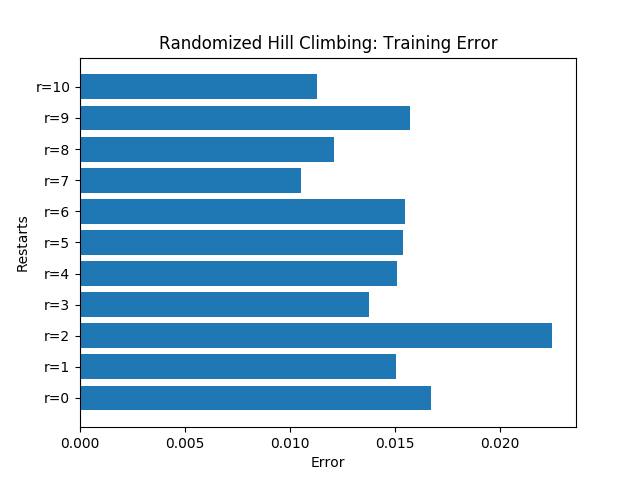
\includegraphics[width=\linewidth]{out/rhc/restarts-training.png}
          \caption{Training error}
          \label{fig:rhc-params-1}
        \end{subfigure}\hfil
        \begin{subfigure}{0.5\textwidth}
          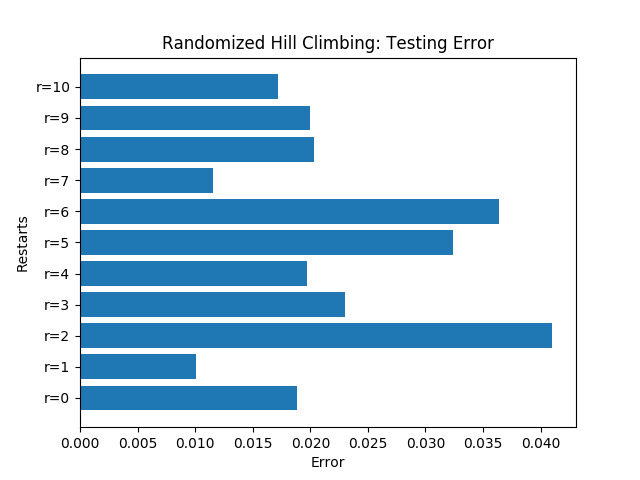
\includegraphics[width=\linewidth]{out/rhc/restarts-testing.png}
          \caption{Testing error}
          \label{fig:rhc-params-2}
        \end{subfigure}

        \caption{Training and testing error for randomized hill climbing with varying restarts.}
        \label{fig:rhc-params}
        \end{figure}

        The results from this test showed that, though the testing error for the various algorithms seemed to trend downward with a higher number of restarts, repeated runs of the algorithm showed too high variance in the error between numbers of restarts to make restarting worthwhile in evaluation.

        Therefore, for the purposes of this data set, it was chosen to not use restarts within randomized hill climbing.

      \subsubsection{Evaluation}
        \Fref{fig:rhc-learning} shows the learning curves for the cancer data set, using randomized hill climbing with no restarts.

        \begin{figure}[htb]
        \centering
        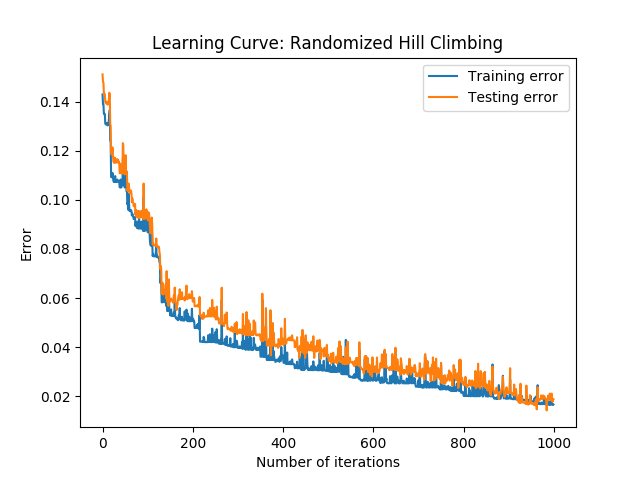
\includegraphics[width=.5\linewidth]{out/plot/RHC.png}
        \caption{Error curves for random hill climbing, with tuned parameters.}
        \label{fig:rhc-learning}
        \end{figure}

        Randomized hill climbing performed well for the cancer data set over a large number of iterations, even without using restarts in weight optimization. Over a larger number of iterations, it may be possible to reduce the training error further, however 1000 iterations was sufficient to reduce the error to a passable level.

        The performance of repeated runs of this algorithm even without random restarts suggest that these data follow a predictable pattern to determine the class of a data point. For 1000 iterations, training time for the randomized hill climbing algorithm was 9.354 seconds with no restarts, and resulted in a 94.161\% testing accuracy.

    \subsection{Simulated Annealing}

      \subsubsection{Parameter selection}
        Simulated annealing, as implemented in ABAGAIL, exposes two hyperparameters: the cooling rate, and the starting temperature. The starting temperature used initially by ABAGAIL was $T = \num{1e11}$, which was sufficient for use, as the cooling rate of the algorithm has a much larger effect on the search. Therefore, the cooling rate was tested at six different values to find the best-performing annealing algorithm after 1000 iterations.

        \begin{figure}[htb]
        \centering

        \begin{subfigure}{0.5\textwidth}
          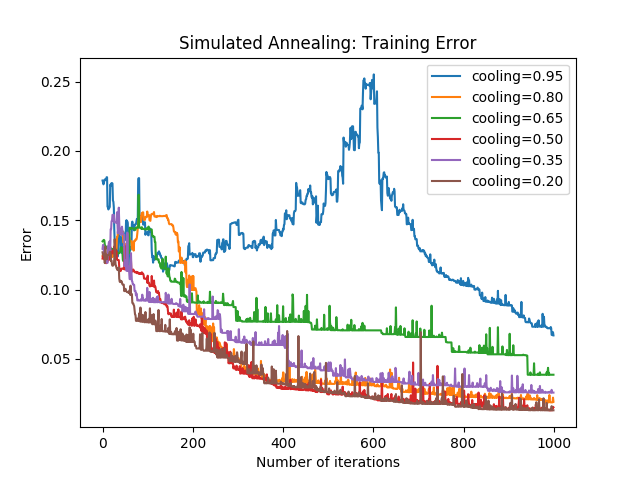
\includegraphics[width=\linewidth]{out/sa/cooling-error-training.png}
          \caption{Training error}
          \label{fig:sa-params-1}
        \end{subfigure}\hfil
        \begin{subfigure}{0.5\textwidth}
          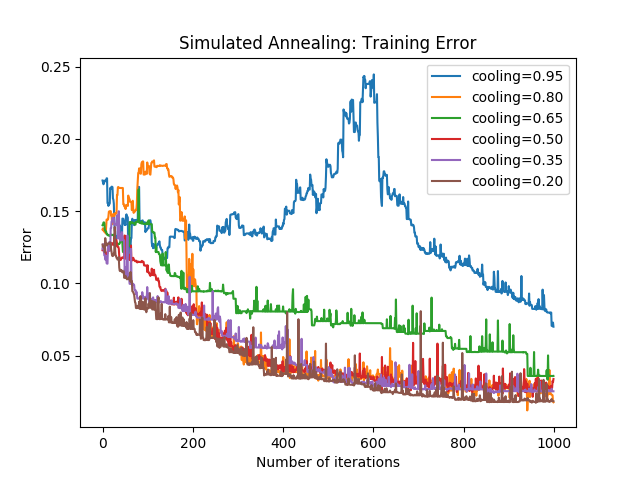
\includegraphics[width=\linewidth]{out/sa/cooling-error-testing.png}
          \caption{Testing error}
          \label{fig:sa-params-2}
        \end{subfigure}

        \caption{Error for simulated annealing with different cooling rates.}
        \label{fig:sa-params}
        \end{figure}

        \Fref{fig:sa-params} shows the training and test error curves for the cancer data set using simulated annealing for weight optimization. The different series in the figure represent different cooling rates.

        The test showed that lower values for the cooling rate, which in turn led to the temperature of the system decreasing faster, performed better on average than numbers for cooling rates. Namely, for both training and testing error, a cooling rate of 0.20 consistently led to lower error at the earlier iterations.

        Interestingly, the algorithm run with $CR = \num{0.20}$ also had the lowest running time with a training time of 7.981 seconds, and the best accuracy with a test accuracy of 95.620\%. Thus, the simulated annealing algorithm was tuned with a temperature $T = \num{1e11}$ and a cooling rate $CR = \num{0.20}$.

      \subsubsection{Evaluation}
        Simulated annealing with tuned parameters was both faster in wall clock time for 1000 iterations than randomized hill climbing, as well as faster to reduce its error. In addition, it resulted in higher testing accuracy than the standard randomized hill climbing algorithm, with a test accuracy of 95.620\% over 94.161\%.

        \Fref{fig:sa-learning} shows the learning curves for the cancer data set using simulated annealing.

        \begin{figure}[htb]
        \centering
        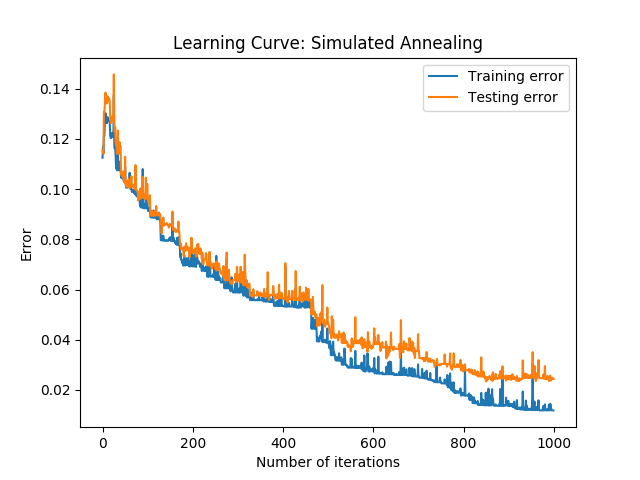
\includegraphics[width=.5\linewidth]{out/plot/SA.png}
        \caption{Error curves for simulated annealing, with tuned parameters.}
        \label{fig:sa-learning}
        \end{figure}

        At a first glance, simulated annealing seems to be a capable alternative to randomized hill climbing that, in this case, is both faster and a better fit. We will explore the effectiveness of hill-climbing algorithms in relation to other alternatives in later sections.

    \subsection{Genetic Algorithms}

      \subsubsection{Parameter selection}
        Genetic algorithms function similarly to populations of organisms, mating and mutating from one generation to the next. The genetic algorithm takes in 3 parameters -- the population site, the number of organisms to mate each generation, and the number of organisms to mutate each generation. Finding a good combination of these three parameters with the best performance is the goal of this section.

        For all runs, the default parameters for testing will be a population size of 200, 50 new organisms being born every generation, and 10 organisms mutating each generation.

        The first parameter of interest will be the population size, with values of 100, 200, and 400. \Fref{fig:ga-population} shows the training and test error curves for the cancer data set using genetic algorithms for weight optimization, varying the population size.

        \begin{figure}[htb]
        \centering

        \begin{subfigure}{0.5\textwidth}
          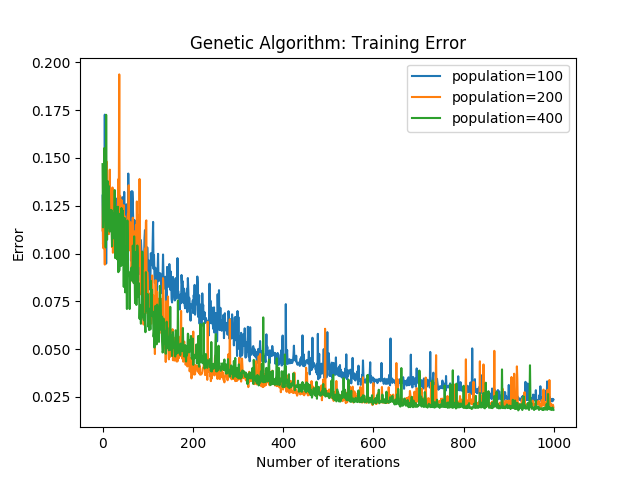
\includegraphics[width=\linewidth]{out/ga/population-training.png}
          \caption{Training error}
          \label{fig:ga-population-1}
        \end{subfigure}\hfil
        \begin{subfigure}{0.5\textwidth}
          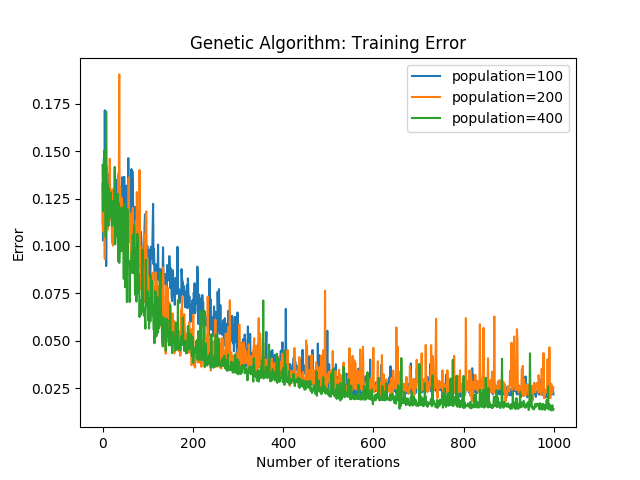
\includegraphics[width=\linewidth]{out/ga/population-testing.png}
          \caption{Testing error}
          \label{fig:ga-population-2}
        \end{subfigure}

        \caption{Learning curves for genetic algorithms with varying population size.}
        \label{fig:ga-population}
        \end{figure}

        In all, population size did not seem to have a drastic effect on the error. The population of size 400 did perform slightly better in terms of error, so a population of size 400 will be used for cross-evaluation of these optimization algorithms.

        Next, the number of new organisms to be born each generation was tested. Mating rates of 25, 50, and 100 new organisms per generation represented an eighth, quarter, and half of the overall population respectively. \Fref{fig:ga-mating} shows the training and test error curves for the cancer data set using genetic algorithms for weight optimization, varying the number of organisms that mate in each generation.

        \begin{figure}[htb]
        \centering

        \begin{subfigure}{0.5\textwidth}
          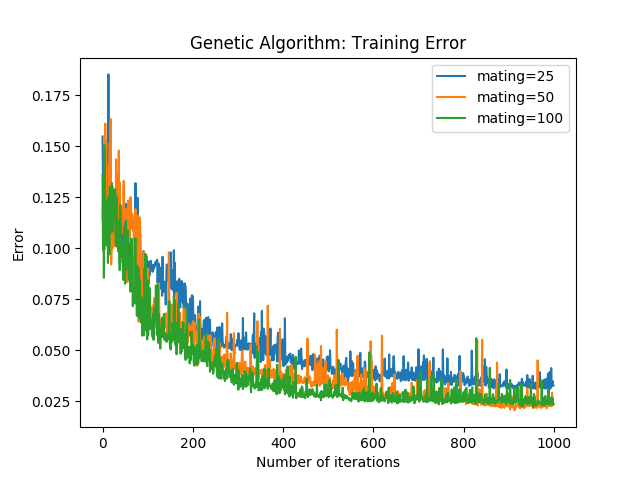
\includegraphics[width=\linewidth]{out/ga/mating-training.png}
          \caption{Training error}
          \label{fig:ga-mating-1}
        \end{subfigure}\hfil
        \begin{subfigure}{0.5\textwidth}
          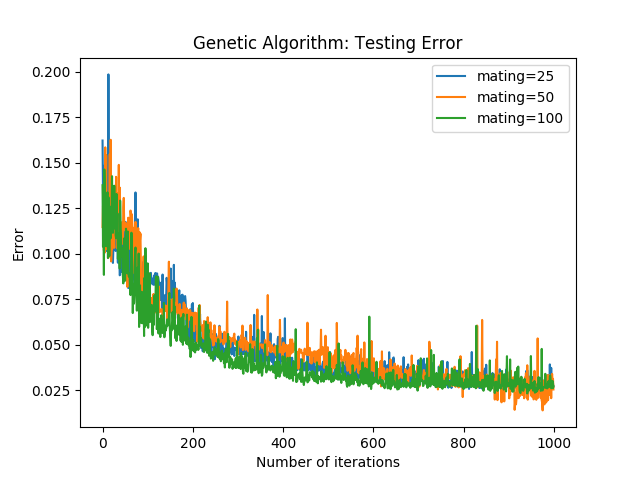
\includegraphics[width=\linewidth]{out/ga/mating-testing.png}
          \caption{Testing error}
          \label{fig:ga-mating-2}
        \end{subfigure}

        \caption{Learning curves for genetic algorithms with varying mating rates.}
        \label{fig:ga-mating}
        \end{figure}

        Testing error was most minimized after 1000 iterations by the test representing mating 50 organisms, or 25\% of the population each generation. Thus, we select a mating rate of 25\%, or 100 organisms per generation with our new population size of 400.

        Lastly, mutation rates were tested with values of 10, 25, and 50 organisms mutating each generation, respectively representing 5\%, 12.5\%, and 25\% of the population mutating respectively. \Fref{fig:ga-mutation} shows the training and test error curves for the cancer data set using genetic algorithms for weight optimization, varying the number of organisms that mutate in each generation.

        \begin{figure}[htb]
        \centering

        \begin{subfigure}{0.5\textwidth}
          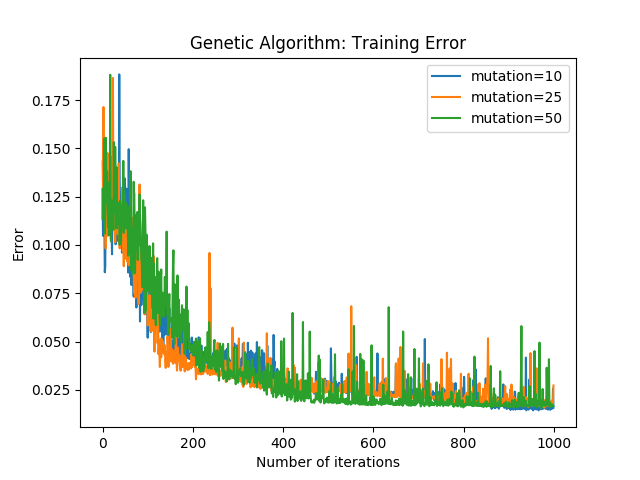
\includegraphics[width=\linewidth]{out/ga/mutation-training.png}
          \caption{Training error}
          \label{fig:ga-mutation-1}
        \end{subfigure}\hfil
        \begin{subfigure}{0.5\textwidth}
          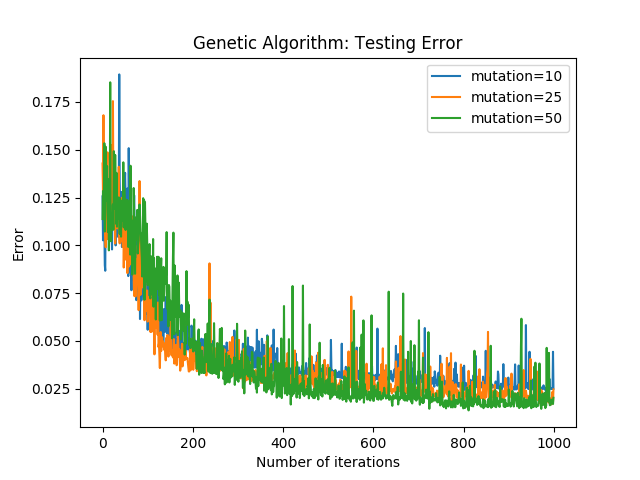
\includegraphics[width=\linewidth]{out/ga/mutation-testing.png}
          \caption{Testing error}
          \label{fig:ga-mutation-2}
        \end{subfigure}

        \caption{Learning curves for genetic algorithms with varying mutation rates.}
        \label{fig:ga-mutation}
        \end{figure}

        Error was again most minimized when mutation rates were 25\% of the overall population. Therefore, we finally select a population size of 400 for our genetic algorithm. With our mating and mutation rates both of 25\%, we configure the algorithm for 100 new organisms to be born each generation, and 100 organisms to mutate.

        In closing, the random nature of the genetic algorithm means that ideally, we would test these parameters over an average of multiple runs to ensure that all parameters were tuned properly. However, in the interest of computing time, this was not done for this assignment.

      \subsubsection{Evaluation}
        In terms of actual test accuracy, the genetic algorithm performed the same as simulated annealing in terms of correct classifications. However, in terms of training error, the genetic algorithm slightly outperformed simulated annealing with a final test error of 0.0210, as opposed to the test error of 0.0244 for simulated annealing.

        \Fref{fig:ga-learning} shows the learning curves for the cancer data set using genetic algorithms.

        \begin{figure}[htb]
        \centering
        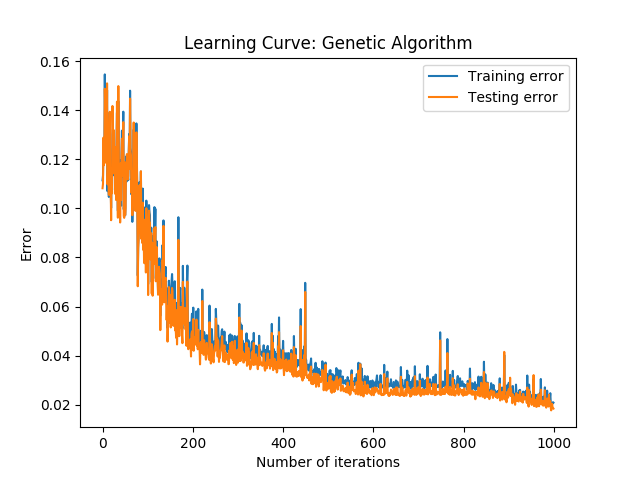
\includegraphics[width=.5\linewidth]{out/plot/GA.png}
        \caption{Error curves for genetic algorithms, with tuned parameters.}
        \label{fig:ga-learning}
        \end{figure}

        It is unclear, with the current test set, whether the genetic algorithm is viable for use over simulated annealing, due to the long runtime of training for a genetic algorithm. This algorithm took a slow 49.519 seconds to train, making the 8.976 second training time of the simulated annealing algorithm preferable.

    \subsection{Comparison}
      After optimization of hyper-parameters, genetic algorithms slightly outperformed simulated annealing and randomized hill climbing after 1000 iterations. After the 1000th iteration, all search algorithms performed similarly, however, the genetic algorithm implementation minimized error at an earlier iteration than in the other two algorithms.

      However, this does not come without a cost. Genetic algorithms, while they did perform well, came at a wall clock time cost, training in a hefty 49.519 seconds as opposed to the 9.354 second and 8.976 second training time over 1000 iterations for randomized hill climbing and simulated annealing respectively. Because the genetic algorithm performed well, a lower number of iterations may be sufficient to improve the runtime of the genetic algorithm without compromising in accuracy, though this would require further tuning to ascertain.

      \Fref{fig:nn-compare} shows the training and test error curves for the cancer data set, using the optimized search algorithms for weight optimization that have been stated in this section.

      \begin{figure}[htb]
      \centering

      \begin{subfigure}{0.5\textwidth}
        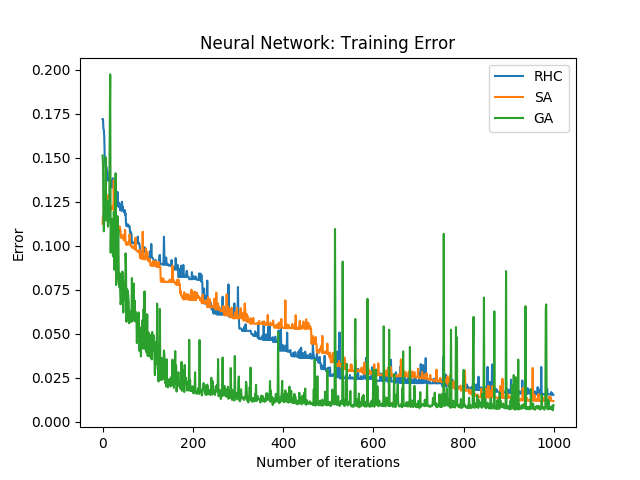
\includegraphics[width=\linewidth]{out/nn-combined-training.png}
        \caption{Training error}
        \label{fig:nn-compare-1}
      \end{subfigure}\hfil
      \begin{subfigure}{0.5\textwidth}
        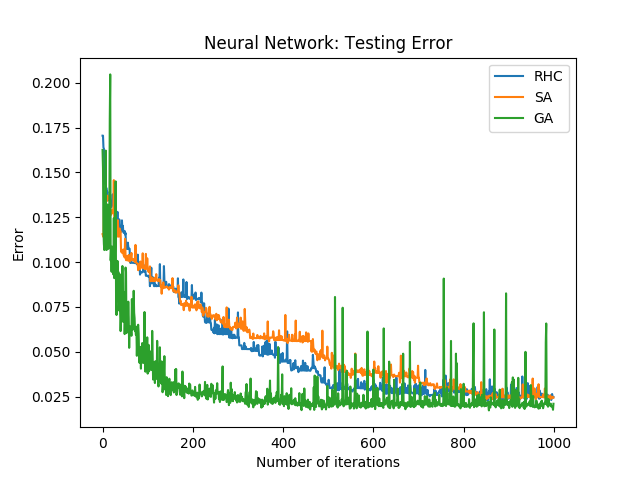
\includegraphics[width=\linewidth]{out/nn-combined-testing.png}
        \caption{Testing error}
        \label{fig:nn-compare-2}
      \end{subfigure}

      \caption{Learning curves for various weight optimization algorithms, with tuned parameters.}
      \label{fig:nn-compare}
      \end{figure}

      However, as \Fref{fig:nn-compare} shows, the genetic algorithm has higher variation in error even after longer training. This extra noise may be a result of the high mutation rate for the genetic algorithm chosen during parameter selection.

      In real world use, it may be possible for the genetic algorithm to be worth use despite the longer training time, but because the slightly better performance comes at a cost of a nearly 400\% increase in training time, the simulated annealing algorithm is the best fit for the cancer data set in the context of this report.

  \section{Exploring Optimization Problems}

    \subsection{Introduction}
      In this section, we will evaluate the three algorithms from the previous section, in addition to the MIMIC algorithm, in the context of three interesting optimization problems. Each algorithm will be tested and compared after 5000 iterations.

    \subsection{Genetic Algorithm: Traveling Salesman}
      The traveling salesman problem is an NP-hard problem that deals with the problem of a salesman traveling from city to city, and returning to their origin city. The goal is to find the shortest route to do so, given a list of cities and the distances between them. The metaphor for this problem extends to many real-world applications, especially in the area of logistics, making it a very interesting problem in the area of optimization.

      \Fref{tab:ts-params} shows the parameters used for each algorithm.

      \begin{table}[h!]
      \centering
        \begin{tabular}{||c|c||}\hline
          \textbf{Algorithm} & \textbf{Parameters} \\ \hline
          Randomized Hill Climbing & N/A \\ \hline
          Simulated Annealing & temperature=\num{1e12}, cooling\_rate=.999 \\ \hline
          Genetic Algorithm & population=2000, mate=1500, mutate=250 \\ \hline
          MIMIC & samples=500, keep=100 \\ \hline
        \end{tabular}

        \caption{Parameters used for the traveling salesman problem}
        \label{tab:ts-params}
      \end{table}

      \Fref{fig:fitness-ts} shows the fitness curve for this optimization problem, comparing the fitness over 5000 iterations for all four algorithms.

      \begin{figure}[htb]
      \centering
      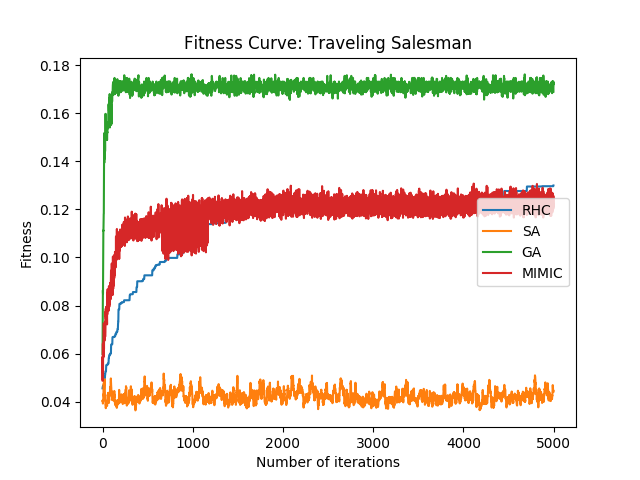
\includegraphics[width=.5\linewidth]{out/op/salesman/fitness.png}
      \caption{Fitness curve for the traveling salesman problem, for various algorithms.}
      \label{fig:fitness-ts}
      \end{figure}

      The genetic algorithm quickly reaches a limit of maximum fitness that majorly outperforms MIMIC and simulated annealing for the traveling salesman problem.

    \subsection{Simulated Annealing: Flip Flop}
      TODO algo talk

      \Fref{tab:ff-params} shows the parameters used for each algorithm.

      \begin{table}[h!]
      \centering
        \begin{tabular}{||c|c||}\hline
          \textbf{Algorithm} & \textbf{Parameters} \\ \hline
          Randomized Hill Climbing & N/A \\ \hline
          Simulated Annealing & temperature=\num{1e11}, cooling\_rate=.95 \\ \hline
          Genetic Algorithm & population=200, mate=100, mutate=10 \\ \hline
          MIMIC & samples=200, keep=20 \\ \hline
        \end{tabular}

        \caption{Parameters used for the flip flop problem}
        \label{tab:ff-params}
      \end{table}

      \Fref{fig:fitness-ff}

      \begin{figure}[htb]
      \centering
      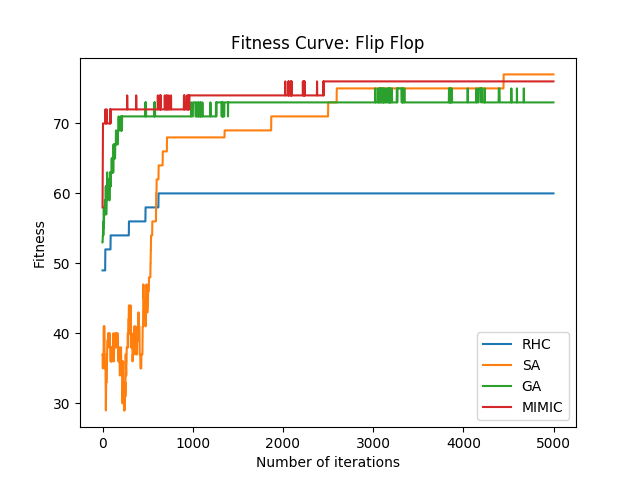
\includegraphics[width=.5\linewidth]{out/op/flipflop/fitness.png}
      \caption{Fitness curve for the flip flop problem, for various algorithms.}
      \label{fig:fitness-ff}
      \end{figure}

    \subsection{MIMIC: Four Peaks}
      TODO algo talk

      \Fref{tab:fp-params} shows the parameters used for each algorithm.

      \begin{table}[h!]
      \centering
        \begin{tabular}{||c|c||}\hline
          \textbf{Algorithm} & \textbf{Parameters} \\ \hline
          Randomized Hill Climbing & N/A \\ \hline
          Simulated Annealing & temperature=\num{1e11}, cooling\_rate=.95 \\ \hline
          Genetic Algorithm & population=200, mate=100, mutate=10 \\ \hline
          MIMIC & samples=200, keep=20 \\ \hline
        \end{tabular}

        \caption{Parameters used for the four peaks problem}
        \label{tab:fp-params}
      \end{table}

      \Fref{fig:fitness-fp}

      \begin{figure}[htb]
      \centering
      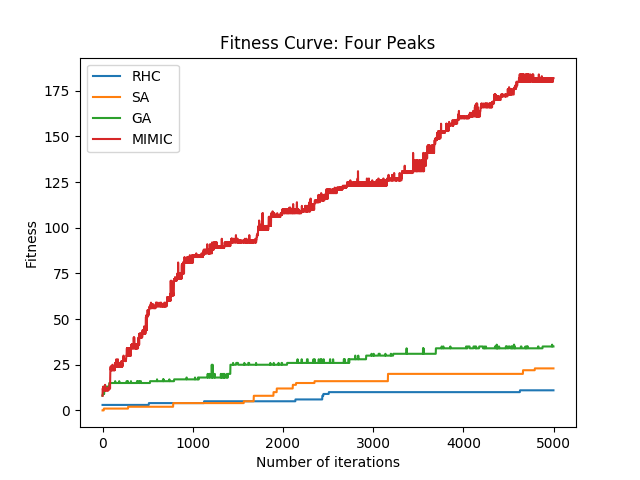
\includegraphics[width=.5\linewidth]{out/op/fourpeaks/fitness.png}
      \caption{Fitness curve for the four peaks problem, for various algorithms.}
      \label{fig:fitness-fp}
      \end{figure}

    \subsection{Discussion}
      TODO

  \section{Conclusion}
    TODO

\end{document}